%preamble
\documentclass[letterpaper]{article}
\synctex=1
\usepackage{graphicx}
\graphicspath{{resources/}}

\usepackage{lipsum}
\usepackage{float}

\usepackage{amssymb}
\usepackage{amsmath}

\usepackage{siunitx}
\usepackage{adjustbox}
\usepackage{multirow}
% for merging table cells I think

\usepackage{tabularx}
\renewcommand\tabularxcolumn[1]{m{#1}}% for vertical centering text in X column

% allows for linewrap within cells
\newcolumntype{Y}{>{\centering\arraybackslash}X}

\usepackage{todonotes}
\usepackage{hyperref}

\usepackage{pdfpages} % for attaching the table lol

\usepackage[section]{placeins} % forces figures to appear in the same section

\usepackage[T1]{fontenc}

%for plots
\usepackage{tikz}
\usepackage{pgfplots}
\pgfplotsset{width=8cm,compat=1.15}\usepgfplotslibrary{patchplots}
\title{ECE 322 \\
Lab Report 3}
\author{Arun Woosaree\\
XXXXXXX}
\begin{document}
\maketitle

\section{Introduction}
The purpose of this lab was to serve as an introduction to mutation testing
techniques, as well as regression testing.

Mutation testing uses the idea of auomatic code mutation to determine how well
the tests a tester writes actually are at catching errors in the application.
The idea is the change, or `mutate' the source code by changing equality
operator, mathematical operaors, among other things. Each copy of mutated code
is referred to as a `mutant', and the same set of tests is run on the mutants.
In order to do the mutation testing, we must first begin with a test suite where
all the tests are green. The idea is that when a mutant fails a test, it is
`killed' and the goal is to make sure that your test suite kills all mutants.
Any mutants that survive are a sign that the tests could be improved, since they
did not catch the bugs the mutants introduced. In this lab, we test an Array
Library program using the mutation testing technique. The program is written in
Java, and was tested using JUnit 5, and the PIT testing library was used to
generate the mutants and evaluate whether they survive the test suite or not.

With regression testing, we are concerned with testing a system again after an
update is made to the code base. For example, when a new feature or `bug fix' is
made, the regression test suite is run to make sure that the change to the code
base does not re-introduce bugs into the system. The idea is that for each
iteration of the software, when a  bug is found, a bugfix is applied, and a test
is also written which checks for that bug. That way, when a new feature is
applied or some other change is made to the codebase, we can make sure that the
new changes do not regress and bring back bugs which were previously already
fixed. In this lab, we test a Math library program using the regression testing
technique. The program is written in Java and a test suite was created with
JUnit 5. 

The project was built using Java 13.
A \textbf{build.gradle} is provided for ease of use,
from which an IDE like Intellij or Eclipse should be able to install
dependencies from and run the tests for both projects. Alternatively, the
command
\texttt{./gradlew test} can be run from the command-line.
\texttt{./gradlew pitest} can be run from the command-line for part 1 of this
lab to generate the mutation test report. 
The test suites for each project are located in \texttt{src/main/test/java}
relative to the project root. 


\section{Task 1}
For part one of this lab, a simple Array Helper library written in Java was
tested using mutation testing. A Java library named PIT test was used to 
generate mutants of the ArrayLib class. Test cases were created which had 100\%
line coverage and branch coverage. These are outlined in the table which can be found in Appendix \ref{part1table}
The failing tests are explained as follows:

\begin{enumerate}
\item \underline{withoutTestRemoveTwo}:
        This test fails because this method depends on ArrayLib's implementation
        of indexOf, which only returns the first occurrence of an element. This
        results in the method only removing one occurrence of a repeated
        element.
\item \underline{withoutTestRemoveFirstElement}:
        This test fails because in the method, there is a check to see if
        $index > 0$, but it should be $index \geq 0$. Because it strictly checks
        for $index > 0$, the first element is never considered for removal.
\item \underline{intersectionTestDuplicate}:
        This test fails because if there are elements that appear more than once
        in both arrays, then the method will attempt to increment the index
        of the intersection array multiple times. However, this array is
        currently limited to the length of array a. To avoid this error, the
        size of the intersection array should be the length of array a plus the
        length of array b. 
\end{enumerate}

To do the mutation testing, the three failing tests above were commented out,
since mutation testing has a prerequisite, which is that the test suite must be
green. With the PIT tool, 37 mutants were created, and 36 were killed. (More on
this later).

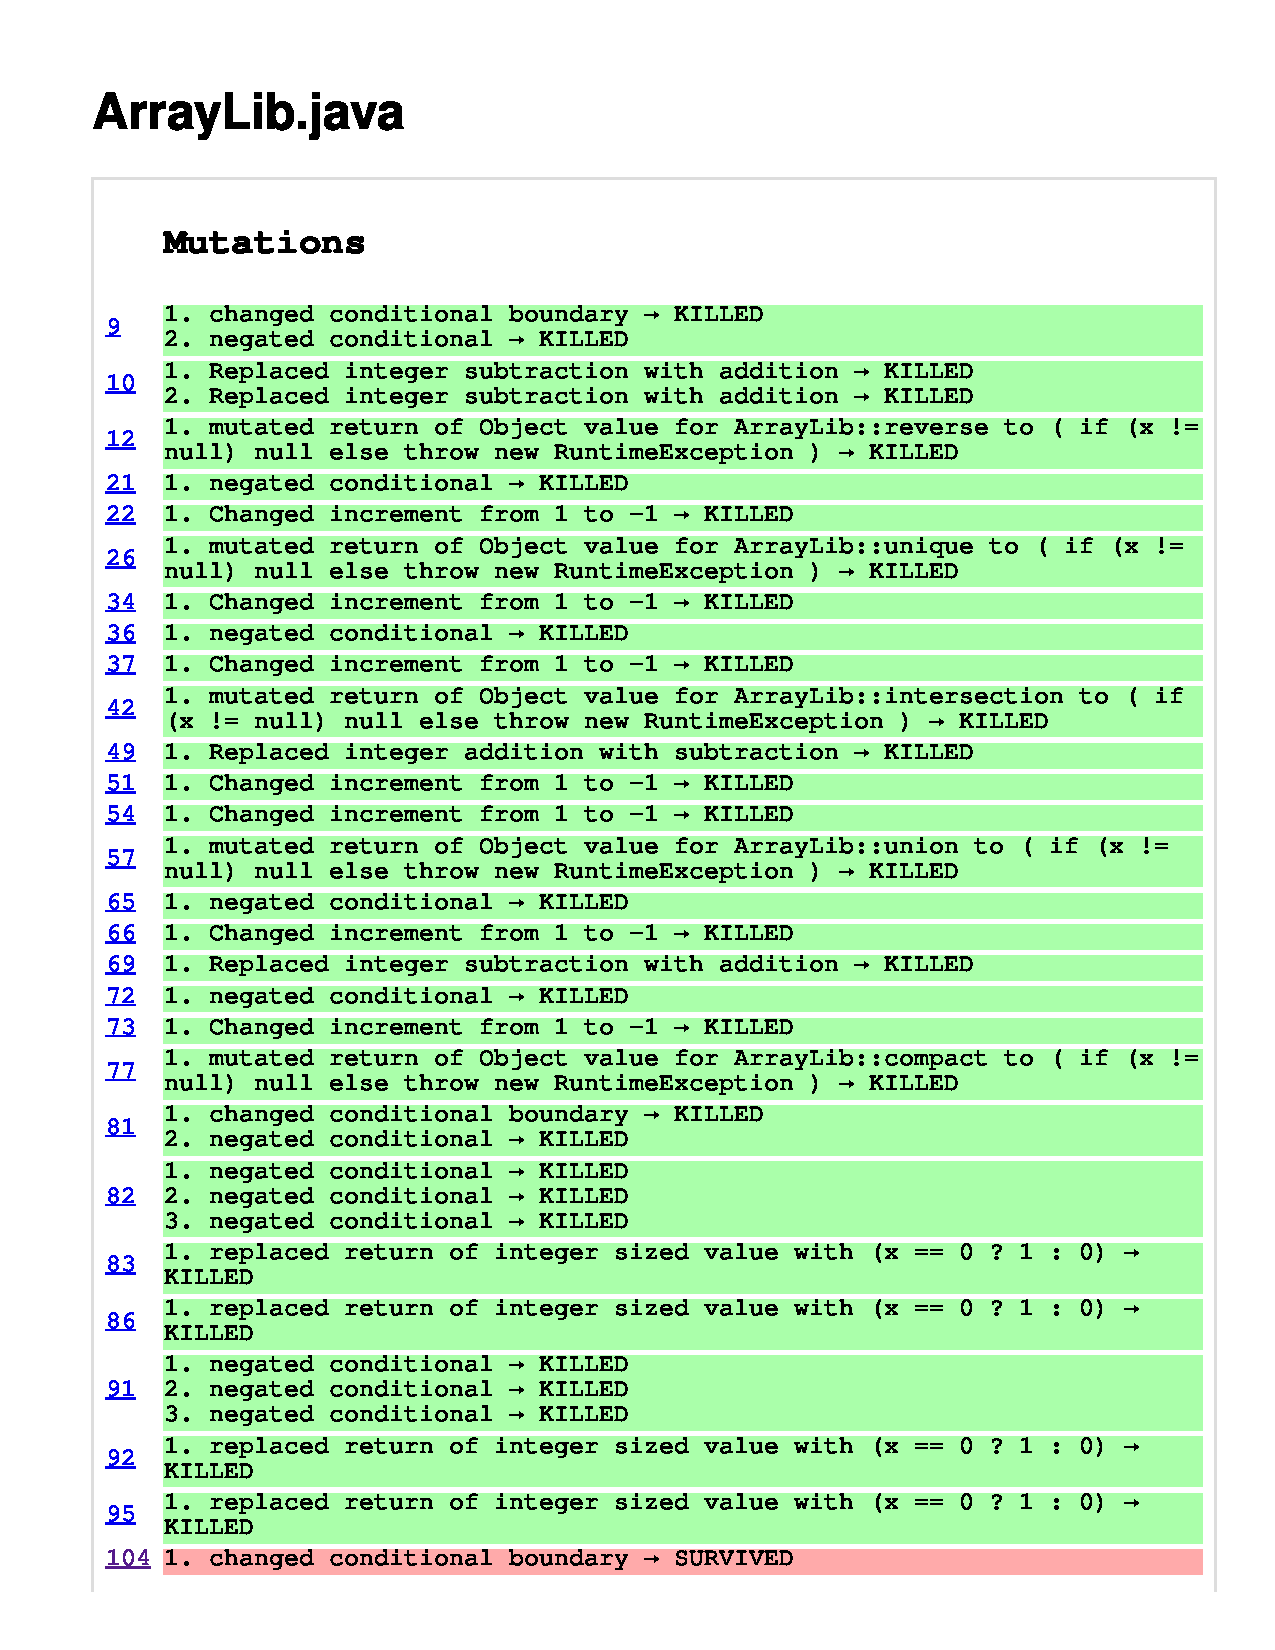
\includepdf[pages=-]{resources/pitest.pdf}

Now, for the one mutant that survived, it is actually directly related to a test
failure mentioned above, which we commented out before running PITest.
Specifically, it has to do with the if statement which checks if $index > 0$
instead of $index \geq 0$ on line 104. 


Before the mutation testing, we found three bugs in the program. After the
mutants were created and killed, only one of the bugs was highlighted by the
mutation test report. In this case, the mutation testing did not expose holes in
the succeeding test cases, but this was mostly due to the luck of the tester
writing good test cases. In other applications, mutation testing can and will
help find holes in weak test suites. This is reinforced by the fact that after
we commented out the failing tests, the mutation test caught one of the bugs
because a mutant survived when the condition on line 104 $index > 0$ was mutated.

I think in the real world mutation testing can be used as an indicator, a sort
of `litmus' test, if you will for the quality of a test suite. It by no means
should be the only thing one checks for to evaluate the quality of a testing
suite, but on its own, it can reveal some weaknesses in a test suite. Like any
other testing strategy, it is not a silver bullet, and the right testing
strategies should be used for the right situations. In general, mutation testing
excels at checking boundary conditions, which can be extremely useful, since
programmers often mix up conditions such as `less than' or `less than or equal
to'.



\section{Task 2}
For the second part of the lab, we are to assume that we have a system with
three independent variables: A, B, C. Each variable has three posisble values:
0, 1, 2. There is no actual testing for this portion, it is a conceptual
exercise.

In total, there are $3 \times 3 \times 3  = 27$ test cases if we were to do
combinatorial testing. We are looking for a standard orthogonal array that
can fit $3^3$. From \url{http://neilsloane.com/oadir/}, we find that
the $L_9(3^4)$ standard orthogonal array works. 
Below is the set of test cases using the orthogonal array mentioned above:

\inputminted{text}{resources/standard3^4}

The PICT program (\url{https://github.com/microsoft/pict}) was used to generate
test cases with the following input:

\inputminted{text}{resources/pict}

It should be noted that strangely, there seems to be different outputs
depending on the operating system that pict is run on.

On GNU/Linux systems, the output is as follows:
\inputminted{text}{resources/pictlinux}

On Windows, the output is as follows:
\inputminted{text}{resources/pictwindoze}

On MacOS, the output is as follows:
\inputminted{text}{resources/pictmacos}

What is strange is that on the Windows and MacOS systems, 10 test cases are
generated, while on GNU/Linux, 11 test cases are generated. 

Given the inconsistent outputs of the pict tool depending on the operating
system that the program is run on, I am not sure about the effectiveness of the
tool for test case generation. Ideally, the test cases generated should be
consistent, since this they are not supposed to be chosen randomly. If the
program worked consistently, however, it would be quite effective since not
much effort would be required to come up with the test cases, and we have the
guarantee that every pair of inputs is tested. 

Compared to the orthogonal array, the pict tool generated more test cases


Pairwise testing is fairly useful, especially when you consider it versus
combinatorial testing. In this toy example, the number of test cases was not
reduced that much, (27 for combinatorial testing, versus 9 with an orthogonal
table), but one can imagine the reduction in test cases when there are more
inputs, and more possible values that these inputs can take on. Compared with
random combinations, pairwise testing gives us the guarantee that we are
testing every single pair of input factors, whereas random combinations
does not have this guarantee, and there are far more combinations to choose
from. However, random combinations can by chance reveal errors that pairwise
testing would not catch.


\section{Conclusion}
In this lab, we were introduced to mutation and regression testing.  We tested
two applications written in Java. The first application is an Array library.
This was tested with the mutation testing strategy, using a library called
PITest. 
In general, mutation testing seems to be a useful tool for getting a feel for
how robust a testing suite is. By generating mutant code, and making sure the
mutants are caught and killed by the testing suite, we gain confidence in the
robustness of the testing suite for each mutant killed. Like any other testing
strategy, it is not a silver bullet, but I can see this technique being used as
a `litmus test' of sorts to give an initial impression for how good a test suite
is. After all, if your test suite does not catch the mutants, and the code base
is later updated when a new feature is added for example and the feature
introduces a bug, the system likely will not work as expected. With a more robust
test suite, it is more likely that changes like this will be caught by the
tests, and therefore won't be introduced to the system. Because computing
mutants takes up a considerable amount of resources, I can see this technique
working well for small to medium-sized systems. I think that for larger systems,
computing the mutants and running the test suites may be too time-consuming.

We also tested a Math application for this lab using the regression testing
strategy. In general, regression testing seems to be really useful for what it
is meant for: making sure previously found bugs are not re-introduced into the
system. I can see it being useful for small and large systems alike. By making
sure known bugs are not reintroduced into the system, developer time and effort
is not wasted dealing with issues more than once, since the tests that cover
each regression test should do the work of catching the bugs as opposed to the
developer trying to trace an issue which was previously fixed before, but some
new feature undid the previous fix. 

Overall, both mutation testing and regression testing techniques seem to be
really useful and practical testing techniques. Mutation testing is more
concerned with the quality of the test suite, while regression testing is
concerned with not re-introducing old bugs, and to prevent regression as the name
suggests. I think that these techniques should not be used alone, but rather
together with other testing techniques learned over the course of the labs.
Making sure your test suite is robust enough to catch small changes is
important, as is the ability to automatically detect and prevent a regression
when a new feature is added to an application. Used in combination with other
testing techniques, these are very powerful. 



\vfill
\appendix

%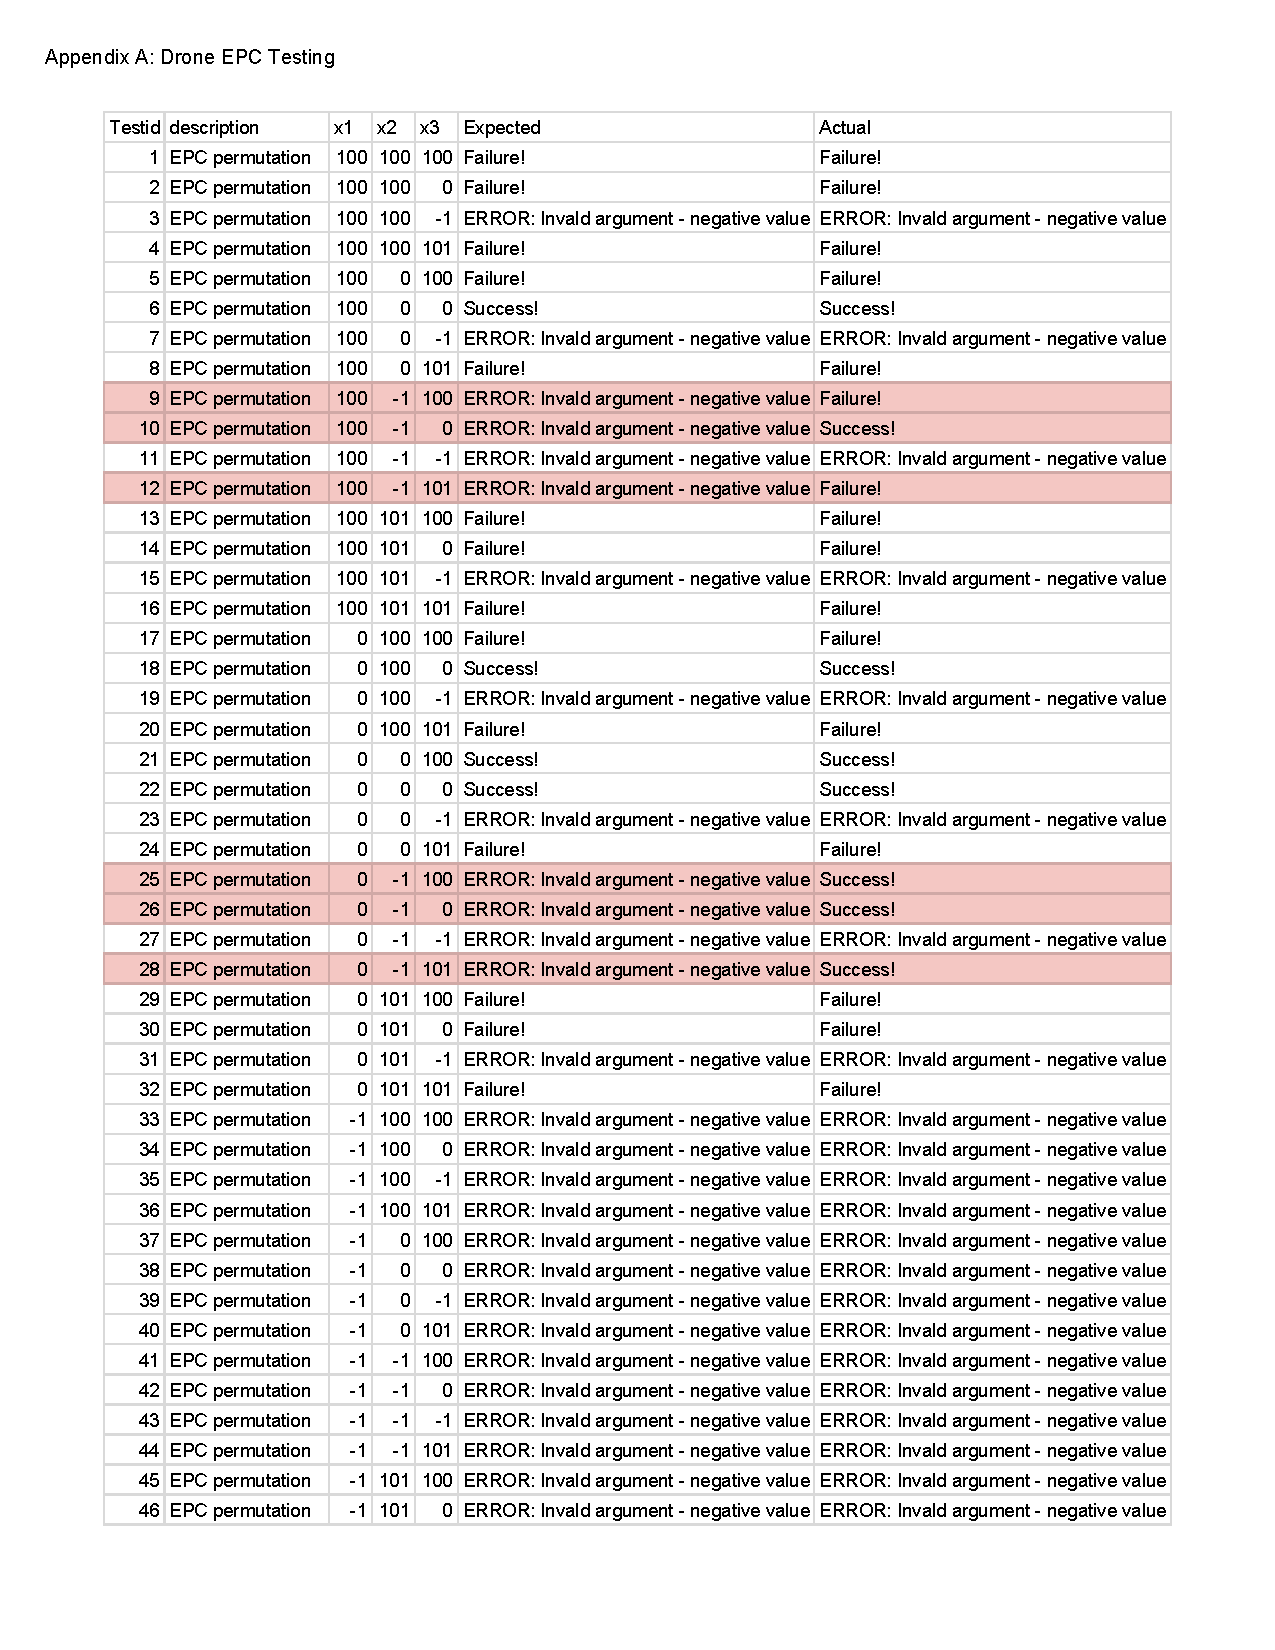
\includepdf[pages=-]{EPC-drone-table.pdf}
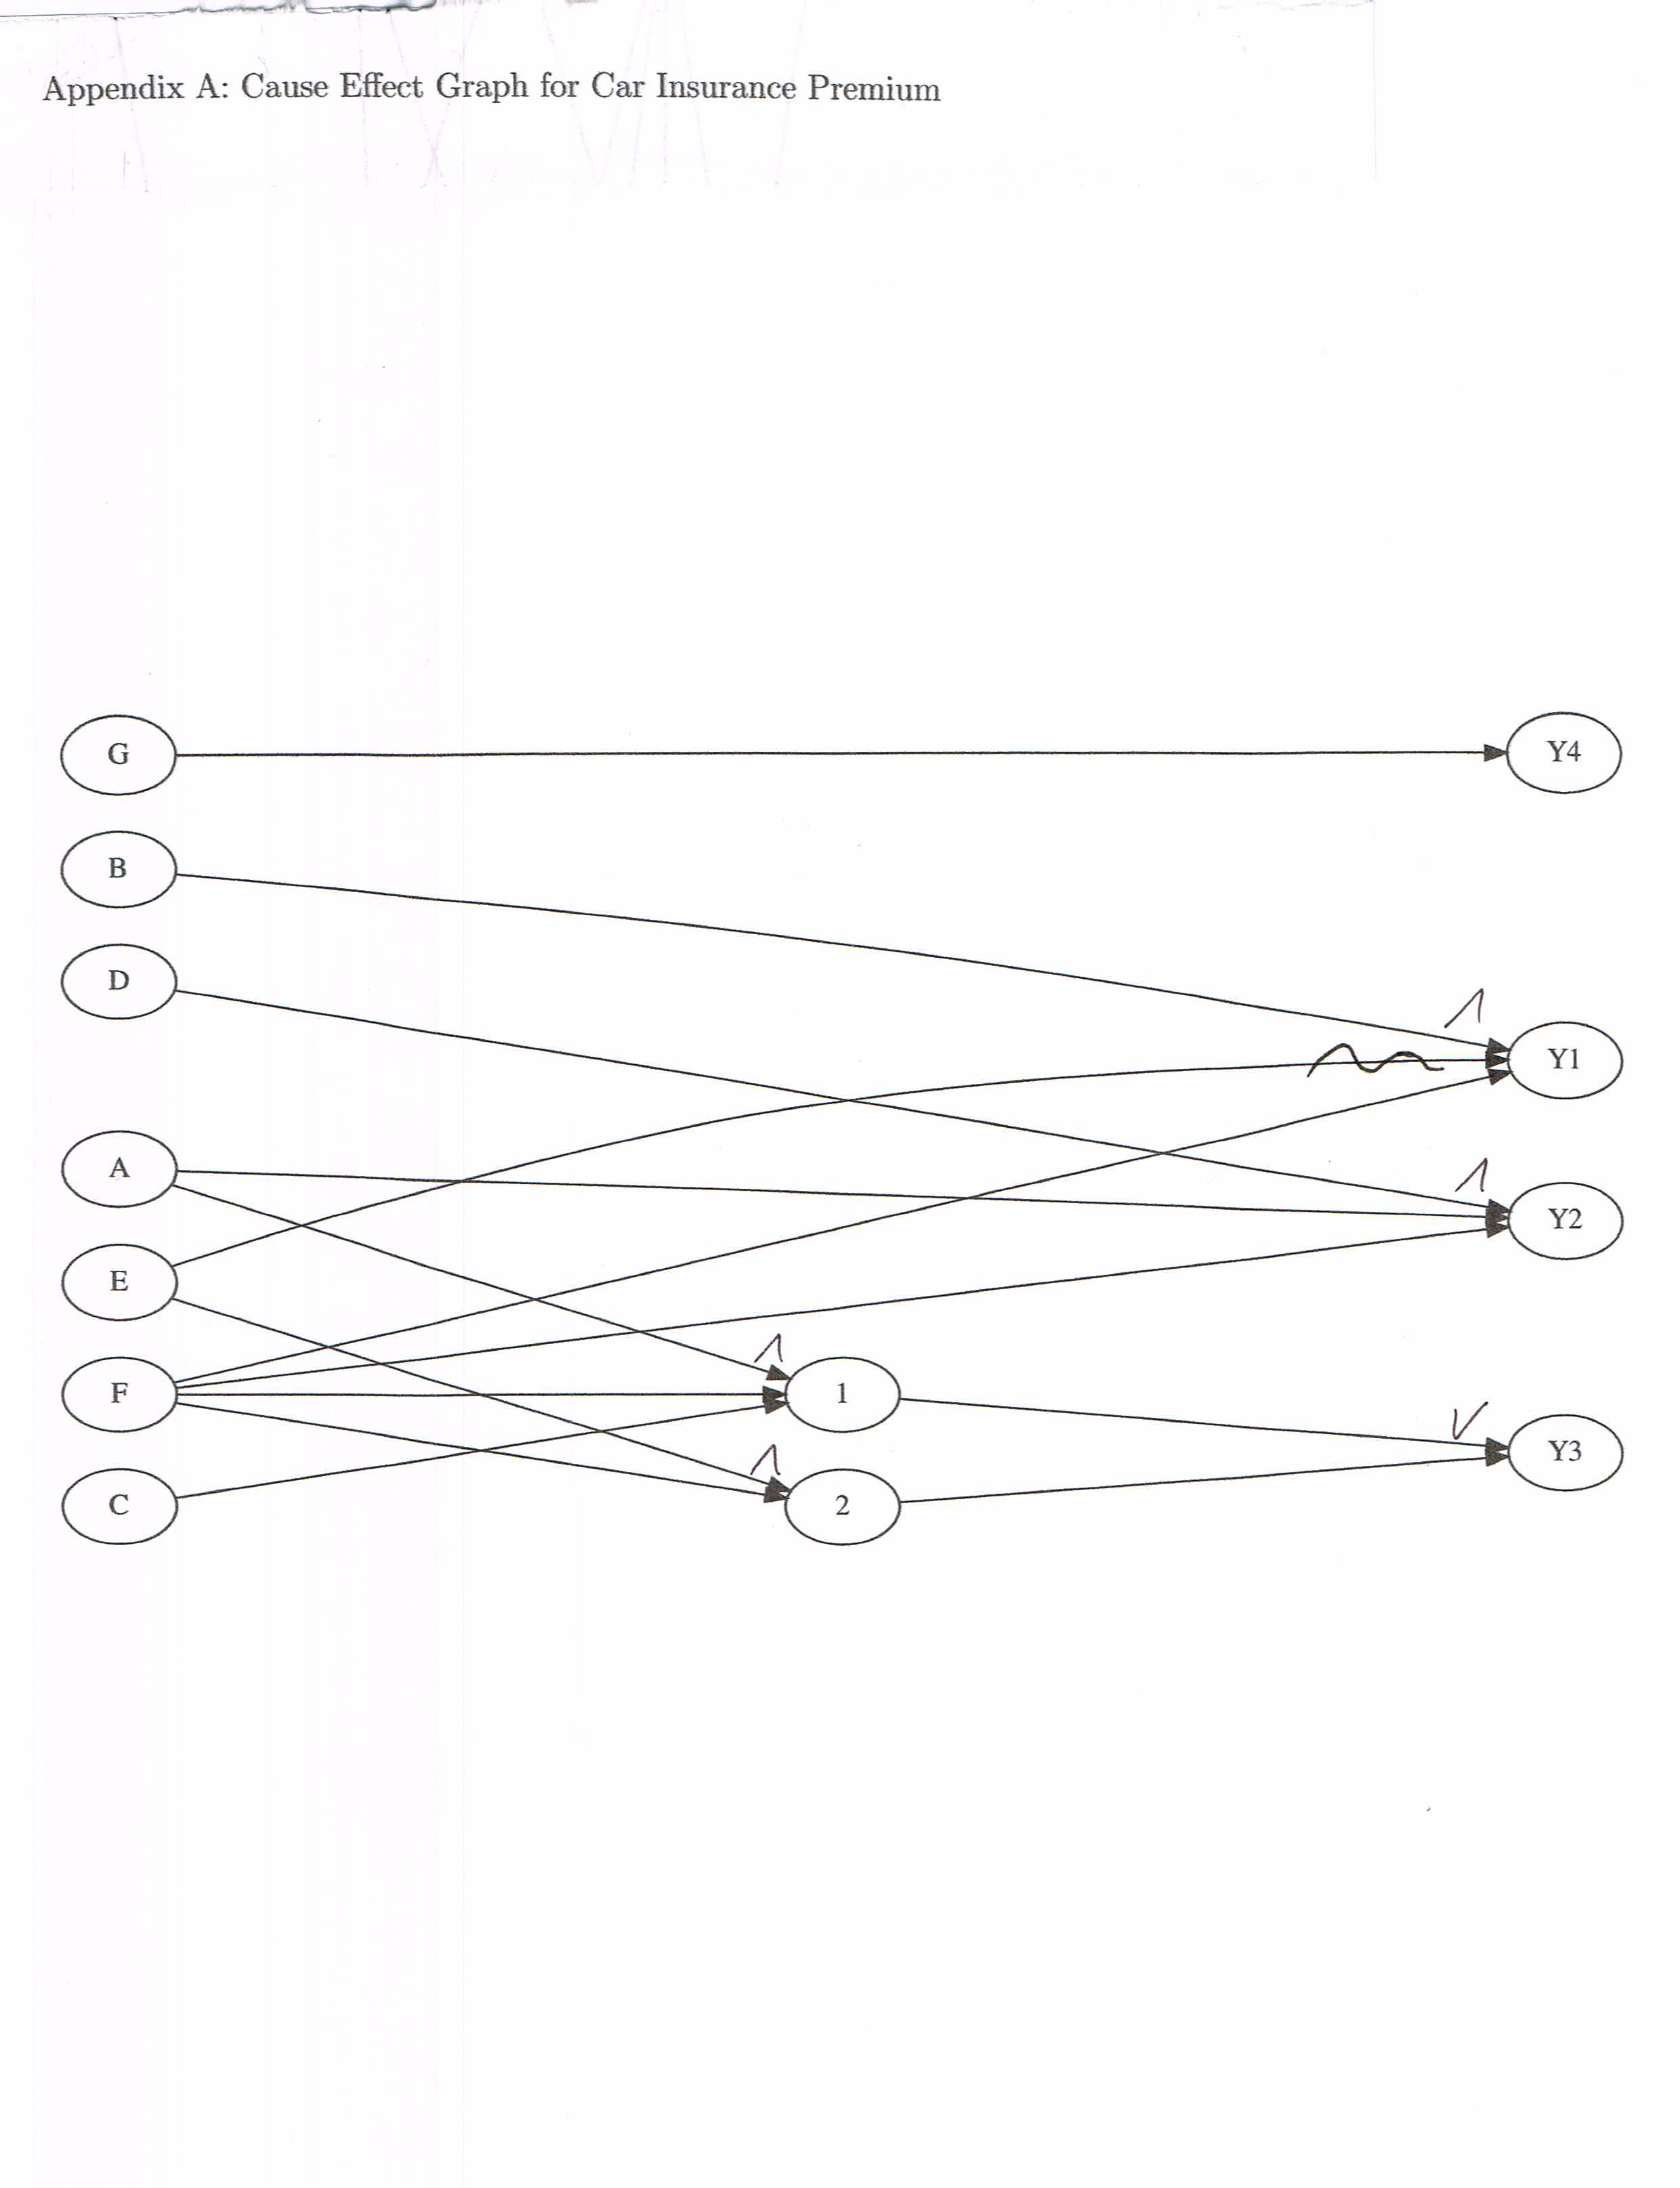
\includepdf[]{causeeffect1.jpg}

%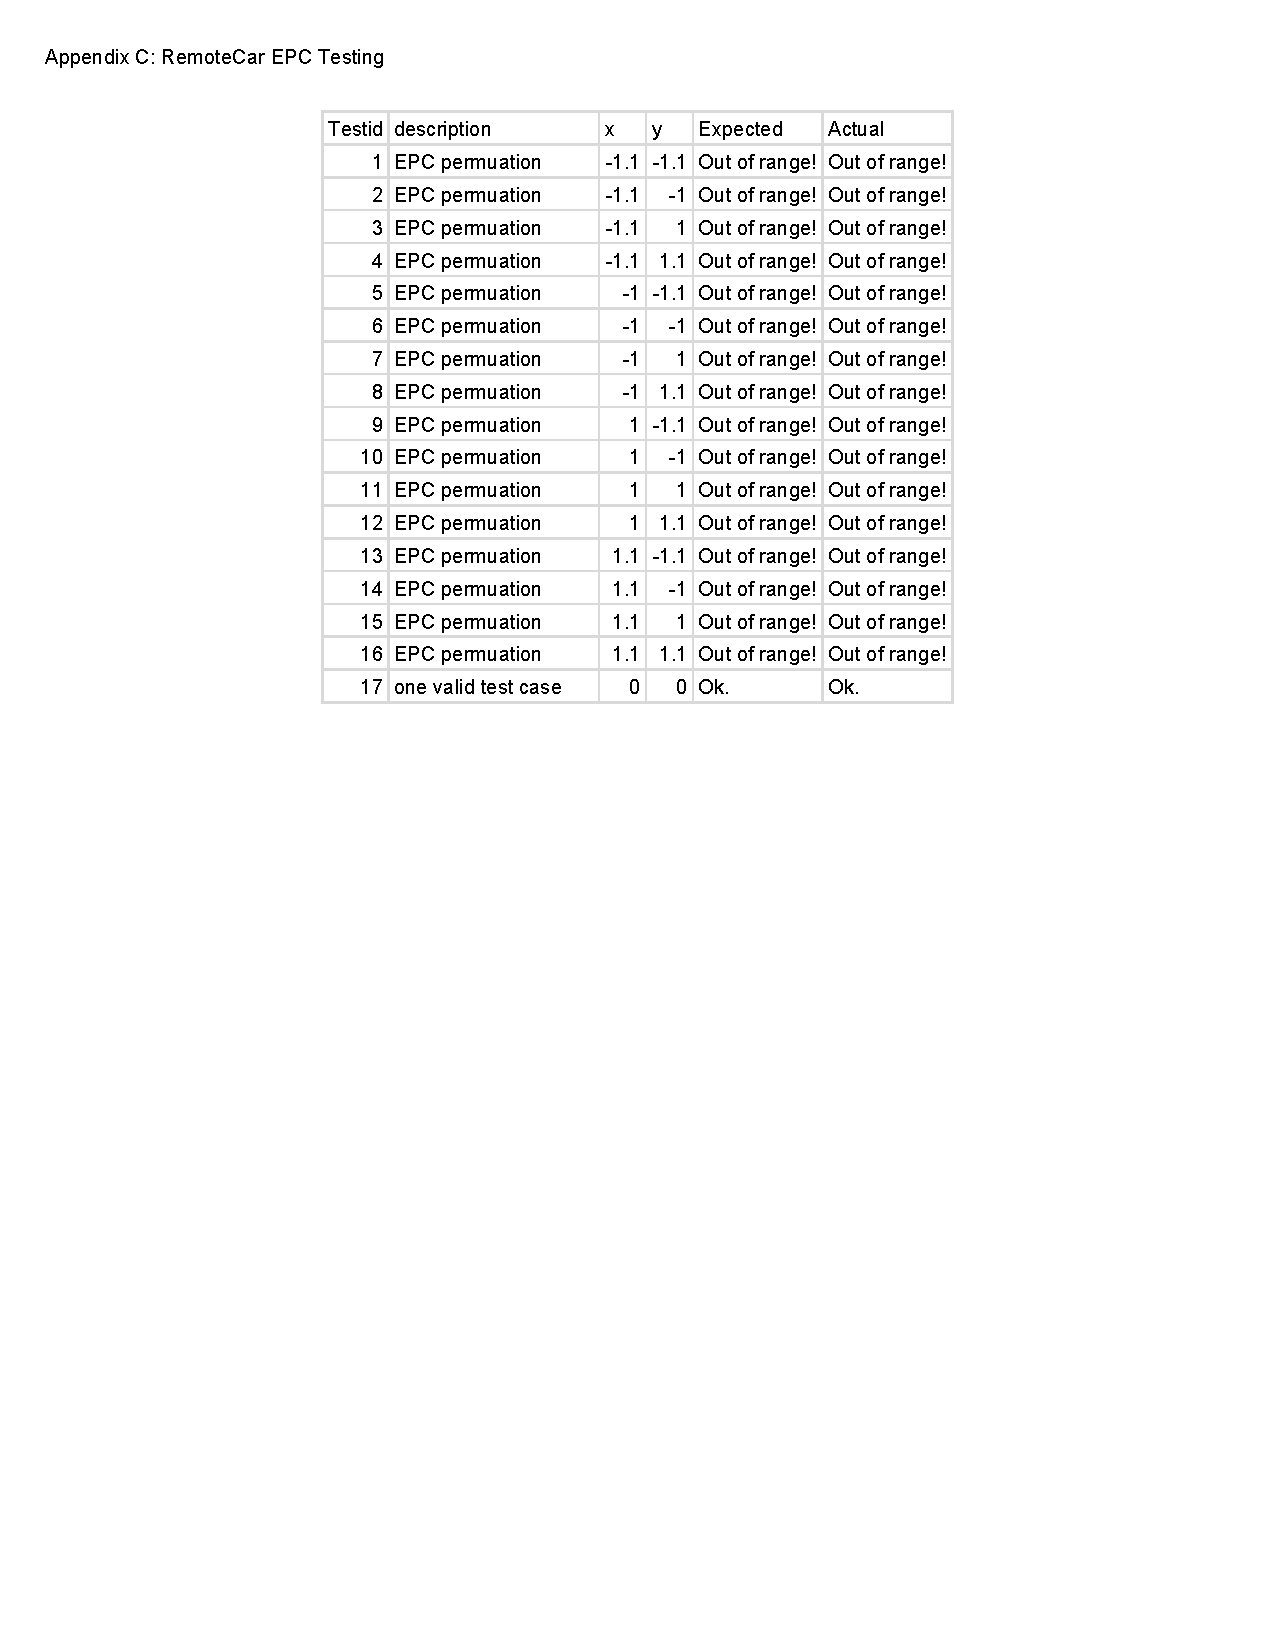
\includepdf[]{EPC-remotecar-table.pdf}
%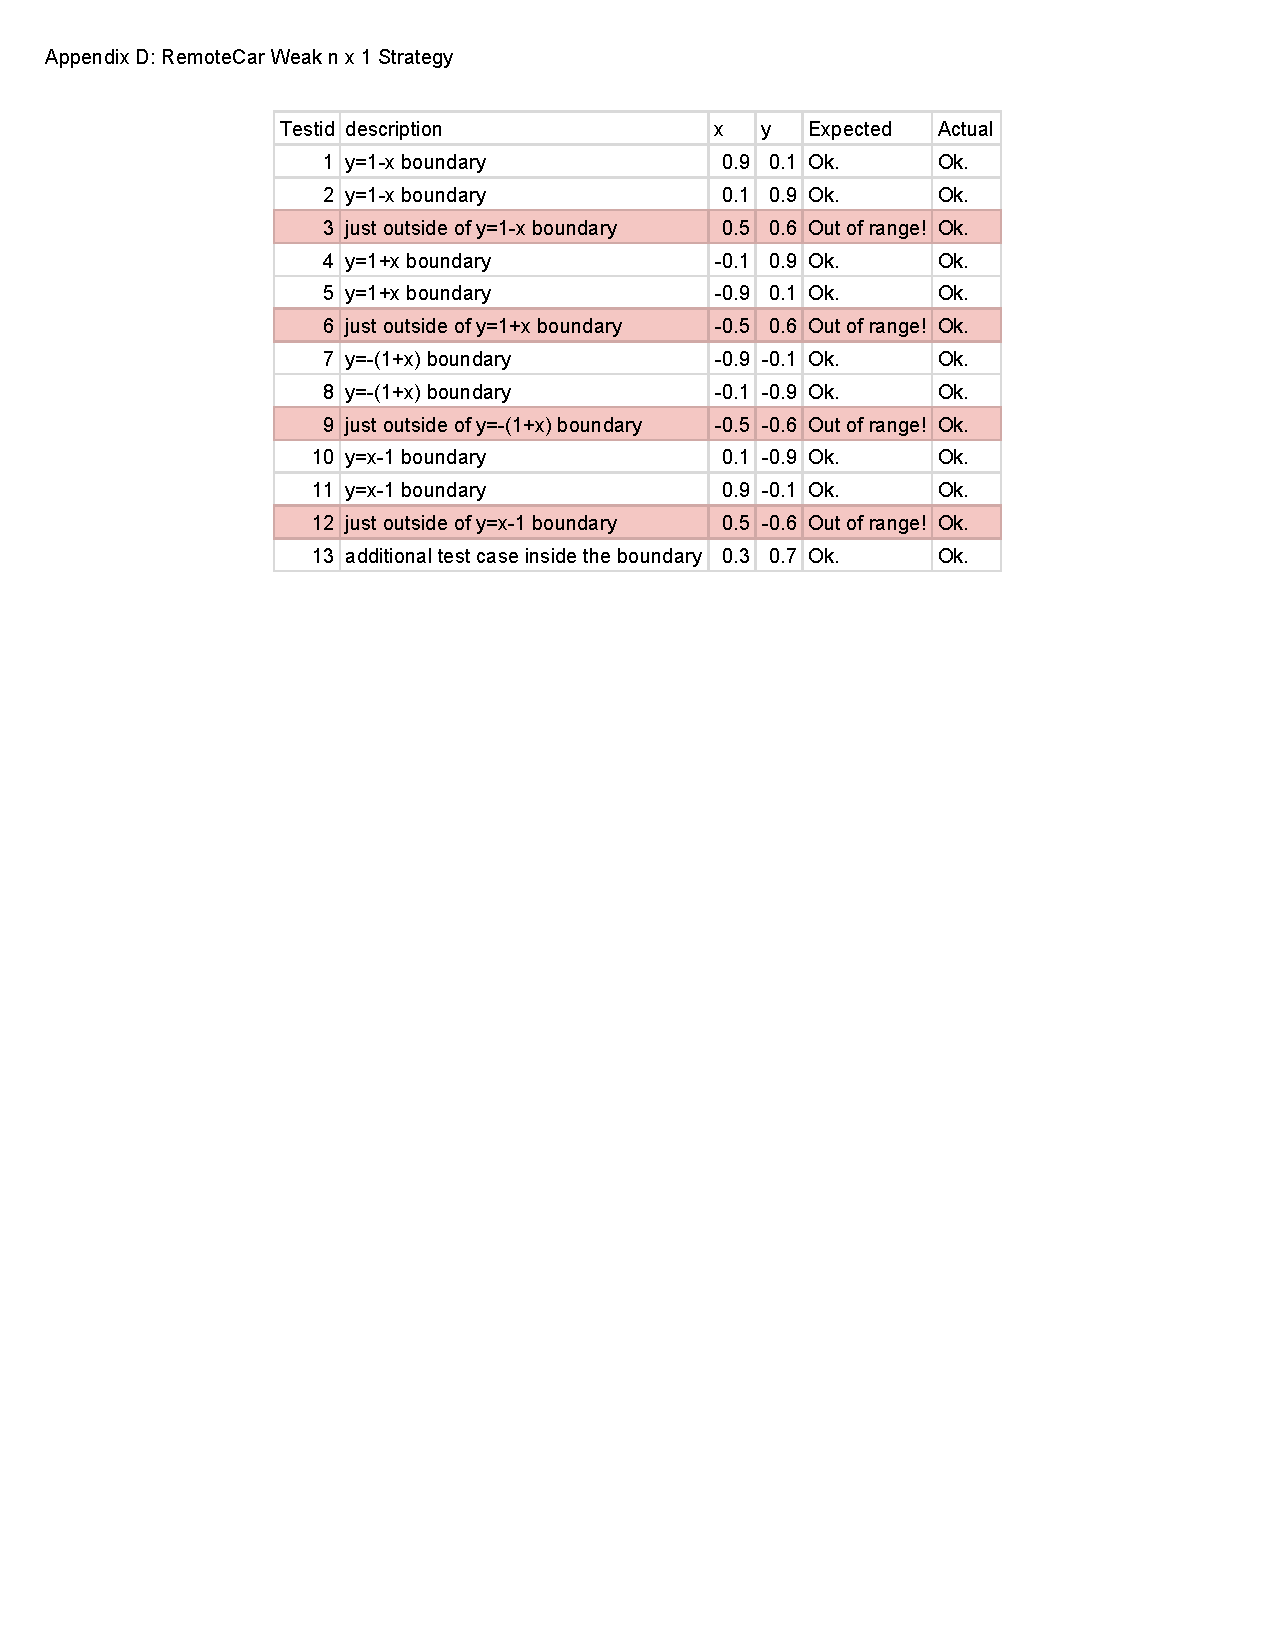
\includepdf[]{weaknx1-remotecar-table.pdf}

\end{document}
